% This is LLNCS.DEM the demonstration file of
% the LaTeX macro package from Springer-Verlag
% for Lecture Notes in Computer Science,
% version 2.4 for LaTeX2e as of 16. April 2010
%
\documentclass{llncs}
%
\usepackage{amsmath}
\usepackage{amssymb}
\usepackage{breqn}
\usepackage{a4wide}
\usepackage{natbib}
\usepackage{tikz}
\usepackage[normalem]{ulem} % for \sout to strikethrough text
\newcounter{instr}
\newcommand{\ninstr}{\refstepcounter{instr}\theinstr.}

\newcommand{\ejmcomment}[1]{{\color{green} #1}}

\newcommand{\mthcomment}[1]{{[\color{red}MTH comment: #1]}}
\newcommand{\mthstrike}[1]{{\color{red}\sout{#1}}}
\usepackage{hyperref}
\hypersetup{linkcolor=blue, citecolor=red, colorlinks=true}


\makeatletter
 \renewcommand\ps@empty{\ps@plain}
\makeatother

\linespread{1.66}
% All text should be double-spaced
% with occasional exceptions for tables. 
%\raggedright
\setlength{\parindent}{0.5in}

\setcounter{secnumdepth}{0}
% Our sections are not numbered and our papers do not have
% Tables of Contents. We don't 
% present a list of figures or list of tables, either.

% Any common font is fine.
% (A common sans-serif font should be used on figures, but figures should be
% separate from the LaTeX document.)

\pagestyle{empty}

\renewcommand{\section}[1]{%
\bigskip
\begin{center}
\begin{Large}
\normalfont\scshape #1
\medskip
\end{Large}
\end{center}}

\renewcommand{\subsection}[1]{%
\bigskip
\begin{center}
\begin{large}
\normalfont\itshape #1
\end{large}
\end{center}}

\renewcommand{\subsubsection}[1]{%
\vspace{2ex}
\noindent
\textit{#1.}---}

\renewcommand{\tableofcontents}{}

\bibpunct{(}{)}{;}{a}{}{,}  % this is a citation format command for natbib
%%for the moment writing up as targeted for sys bio software paper
%Software for Systematics and Evolution Articles
%Submissions should describe new or original software or tools that provide new analytical capabilities to the end user. 
%Submissions may also be considered that describe new versions of existing software, 
%provided that the new version makes significant changes to function or performance 
%(for example, a version that implements new and important methods in addition 
%to those previously provided in a software package might be considered for publication). 
%Publication will be determined largely based on the software or tool itself, 
%so working links to a functional copy must be provided at the time of submission.
%Additional requirements: 
%The software or tool must well documented and easy to use for the typical user. 
%The manuscript itself must be readable by the general Systematic Biology readership. 
%If relevant, the manuscript must include benchmark data, 
%or refer to Supplemental Material that includes such data. 
%If appropriate, such benchmarking should include real biological data and a comparison with related tools. 
%If appropriate, the submission must include working sample data files. 
%Any software must be open source, web-distributed and free to non-commercial users. 
%In addition, the authors must certify that they will provide support 
%for the software or tools for a minimum of two years from the date of publication. 
%Systematic Biology encourages the use of GPL-like licenses and the use of open repositories, such as SourceForge or Google Code.
%Software for Systematics and Evolution papers should include an abstract. 
%In general, papers will be limited to 4 printed journal pages (less than 12 double-spaced manuscript pages), 
%but exceptions can be made when warranted. We will not enforce any specific organization of the text, 
%but the following suggestions might help in organizing a submission: an introduction that describes the motivation; 
%a Description section; a Benchmark section; a Biological Examples section (if applicable); a statement regarding Availability. 
%However the manuscript is organized, please pay careful attention to the normal formatting 
%for section headings, references, and other aspects of the journal’s style.

\begin{document}
\begin{flushright}
Version dated: \today
\end{flushright}
\bigskip
\noindent RH: Speed dating


\bigskip
\medskip
\begin{center}

% Insert your title:
\noindent{\Large \bf A dynamic programming approach and tool for speed-dating and divergence time estimation}
\bigskip

% We don't use a special title page; the author information is entered 
% like any other text.

% FOOTNOTES: We don't allow them in the manuscript, except in
% tables. Don't include any footnotes in the text.


\noindent {\normalsize \sc Tom\'{a}\v{s} Flouri$^1$, Emily Jane McTavish$^{1,2}$, Diego Darriba, Pashalia Kapli, Mark T.\@ Holder, Alexandros Stamatakis$^{1,3}$}\\
\ejmcomment{We haven't discussed order AS: I personally don't care, maybe Mark should go last due to more closer involvement\\ Email Bastien about further involvement? AS: not sure 
how much he really contributed or is able to contribute.\\}
\noindent {\small \it 
$^1$Heidelberg Institute for Theoretical Studies, Heidelberg, 69118, Germany\\
$^2$Ecology and Evolutionary Biology, University of Kansas, Lawrence, KS, 66045, USA\\
$^3$Institute of Theoretical Inofrmatics, Karlsruhe Institute of Technology, Karlsruhe, 76131, Germany}
\end{center}
\medskip
\noindent{\bf Corresponding author:} Tom\'{a}\v{s} Flouri, 
Heidelberg Institute for Theoretical Studies; Heidelberg, 69118, Germany, E-mail: Tomas.Flouri@h-its.org.\\

% Of course the specific format of addresses may vary according to
% country or other factors. Also, that was just an example email format.
%It's acceptable to add email addresses for authors in addition to the
%corresponding author. These would be placed after "Country."

\vspace{1in}

\subsubsection{Abstract} We present a dynamic programming algorithm to rapidly
date phylogenies with thousands of tips and make it available in the open source software package FastDate. 
Our tool can use prior information on node or tip dates to either scale trees to absolute time.
If this information is not available, FastDate can alternatively estimate relative times for nodes.
We have integrated recent mathematical models to calculate tree probabilities {\bf TODO tree probabilities sounds as if we are samoling over trees which we are not} 
that account for
incomplete  sampling of extant as well as ancestral species.
This incomplete sampling can be due to fossilization and recovery processes, for instance.
{\bf TODO add results, speed and comparison to established programs for dating!}
FastDate is \ejmcomment{(will be)} available as a web-service at {\bf TOOD} and open source code at {\bf TODO}.\\
\noindent (Keywords: )\\

\vspace{1.5in}

Phylogenetic analyses produce trees with branch lengths that represent the expected number of substitutions per site.
Each branch length is a product of a lineage's substitution rate and elapsed time.
To generate time\textendash scaled trees it is necessary to disentangle the time from the substitution rate.
Answering  a plethora of biological questions does require time\textendash scaled trees.
Phylogeographic and paleontological analyses depend upon node dates in absolute time,
to associate evolutionary with historical events.
Identifying changes in diversification rates and inferring causes for those changes
rely on accurate estimates of relative speciation times.
As recent sequencing and computational developments allow to infer
phylogenies with thousands of tips, rapid approaches for dating such trees are needed.

The most straightforward approach to dating trees is to use the molecular clock model.
It assumes that the rate of nucleotide substitutions is constant through time \citep{zuckerkandl1962}.
However, due to both stochastic variation in observed mutations and 
biological variation in rates of mutation fixation across different lineages,
using a strict molecular clock does typically not generate an ultrametric tree.
Several alternative approaches have been developed to estimate
ultrametric trees using relaxed clock or correlated rates {\bf TODO rate or rates?} models \citep{Lepage2007, Thorne1998, Kishino2001}.
In order to anchor branch length estimates in absolute time, researchers deploy so-called calibration dates. 
There are two main approaches to annotate phylogenies by absolute times:
priors on node ages or tip dates.
Node priors are probability distributions on the ages of nodes {\bf TODO do you mean inner nodes of the tree or does this refer to all nodes?}.
These node age estimates are often obtained from fossils,
but can also be inferred from geological, biogeographical, or other external information.
Tip dating approaches are usually applied to serially sampled data, that is, 
data where some tips were sequenced in the past, and have known sequencing dates.
While tip-date information is most commonly used in bacterial or viral phylogenies,
it is also possible to use fossil taxa as tips.
Tip dates may either be prior distributions or fixed, dsicrete dates, 
depending on the sampling {\bf not clear what you mean by sampling here} and the uncertainty associated with the respective
dating technique.
\citet{Heath2014} developed the fossilized-birth-death model which 
uses an explicit macroevolutionary model to integrate over potential 
placements of fossils {\bf TODO define what you mean by fossil placement, is this in the entire tree or just along a branch?} for dating phylogenies.

Irrespective of the date information type, reconciling {\bf TODO is there a better word than reconciling, previsouly you used calibrating, are those words used as synonyms?} 
multiple calibrations dates with branch lengths across a tree with more than a few tips represents a challenging task.
Several Bayesian methods have been developed which use Markov Chain Monte Carlo (MCMC) methods
to infer dated phylogenies using prior information, 
(e.g. BEAST \citealt{Drummond2007}; BEAST 2 \citealt{bouckaert2014}; MCMCTree \citealt{Stadler2013}).
While these approaches can be accurate, and integrate over uncertainty about the dated
phylogeny {\bf TODO need to more accurately describe what you mean with ``integrate over uncertaionty about the dated phylogeny''}, 
for trees with many tips or many calibration points, they can be intractably slow.
{\bf Add a sentence that they (Beast for sure, not sure what MCMCTRee does) rely on calculating likelihoods on tree and data,
thus they are also slow for very large phylogenomic datasets, i.e., the performance bottleneck are always the likelihood calculations!}
For example, using BEAST to estimate the dates for the phylogeny in \citet{Misof2014}, which has 144 tips
and 37 node calibration priors, entailed thousands of CPU hours.{\bf TODO can we be a bit more specific here? Was it possible to date the tree using the entire dataset?}

Some rapid phylogenetic dating approaches have been developed which do not rely on MCMC and on associated phylogenetic likelihood calculations on the alignments.\@
R8s uses non-parametric rate smoothing to rapidly estimate 
maximum likelihood calibrated or ultrametric trees \citep{Sanderson2003}.
Least Squares Dating (LSD) (REF Gascuel) 
\ejmcomment{Need to cite but it isn't publicly available anywhere.}{\bf TODO shall I ask him where we can find/ho wto cite it?}
uses a least squares approach based on a normal approximation of the molecular clock.
<<<<<<< HEAD
According to (Gascuel LSD ref) LSD achieves similar results to BEAST but is orders of magnitude faster. 
\cite{Akerborg2008} describe a dynamic programming-like approach to 
rapidly generate ultrametric phylogenies from an input tree topology.
The approach uses discretization of the time scale.
A standalone, open source implemention of this algorithm is not available,
but it is implemented as a part of the PrimeGSR program \citep{Akerborg2009}.{\bf is PrimeGSR open-source?}


Our program, FastDate, is adapted from the algorithm in \cite{Akerborg2008}.
FastDate implements a faster version of the dynamic programming approach running 
in quadratic time as a function of the number of bins of the time scale;
the original algorithm ran in cubic-time.
FastDate produces an approximation of the maximum {\em a posteriori} (MAP)
estimate of the ages of node of a sampled tree.
Similar to the original algorithm of \cite{Akerborg2008}, FastDate treats
the branch lengths in terms of expected substitutions per site as known without error.
FastDate uses priors on node ages of sampled trees conditional on the 
number of extant tips sampled derived in \cite{Stadler2010}.
The rate of molecular evolution on each edge is assumed to follow a 
gamma distribution, as in the uncorrelated model of \cite{BEASTREF-FOR-THIS-MODEL}.
FastDate can use prior information on node dates or tip dates as additional
factors in calculation of the posterior probability density.
The user can choice of the number of time intervals to which 
nodes can be assigned, which controls the granularity of the approximation.
The user must also specify a maximum possible root age.


\section{Methods}

\section {Preliminaries}
%
%
\subsection{Basic definitions}

%
A tree $T=(V,E)$ is a connected acyclic graph where $V$ is the set of {\em
nodes} and $E$ the set of {\em edges}, such that $E = V\times V$. We use the
notation $(u,v) \in E$ to denote an edge with end-points $u,v \in V$. If $T$ is
{\em oriented}, $(u,v) \in E$ indicates that the edge originates at $u$ and leads
to $v$, in which case $u$ is called the {\em parent} and $v$ the {\em child}.
The {\em in-degree} (resp.~{\em out-degree}) of a node denotes the
number of incoming (resp.~outgoing) edges of $u$. The
{\em degree} of a node $u$ denotes the number of edges $u$ is an end-point of.
We denote with $T_u$ the subtree of $T$ rooted at node $u$.  A {\em
rooted binary tree} $T$ is a {\em directed} tree with all nodes having
in-degree $1$ and out-degree $2$ ({\em inner} nodes), or in-degree $1$ and out-degree
$0$ ({\em leaves}). The single root node has in-degree $0$ and out-degree $2$.  
Henceforth, we use the term tree to denote a
binary rooted tree.  We refer to the set of leaves of tree $T$ as $L(T)$.  The
cardinality of a set $X$ is denoted as $|X|$. The {\em height} $h(u)$ of a node
$u$ of $T$ with children $v$ and $w$ is defined as 
%
\[ h(u) = \left\{ \begin{array}{ll}
\max(h(v), h(w)) + 1 & \quad : \quad u \notin L(T)\\
1                    & \quad : \quad u    \in L(T)\\
\end{array}\right. \] 

{\bf TODO why shouldn't the height of the leaf nodes be set to zero? you should explain that this might be needed later on}

The height $h(T)$ of a tree $T$ is the height of its root. Finally, the mapping $\ell : E \mapsto \mathbb{R}$ maps
each edge to a real number which we call the {\em branch length}, and we will use the notation $\ell_{u,v}$ for
the branch length of edge $(u,v)$.

\subsection{Branch rate distribution}

\mthcomment{I think that we can just say that we use uncorrelated Gamma rates, and delete this section.}

Setting dates on a tree requires factorizing the branch lengths of an input topology
from estimates of evolutionary distances into rates and times. 
A common approximation is to treat branch rates as gamma distributed \citep{Kishino2001}.


The {\em Gamma function} is an extension to the factorial function that accepts
real or complex numbers as arguments. For point $t$ it is defined as
$$\Gamma(t) = \int_0^\infty x^{t-1} e^{-x} dx.$$

The {\em probability density function} in the shape-rate parameterization of a
{\em gamma distribution} given the {\em mean} $\mu$ and {\em variance} $\sigma^2$ 
is
$$ \gamma(x;\alpha,\beta) = \frac{\beta^{\alpha}x^{a-1}e^{-x\beta}}{\Gamma(\alpha)} $$

where $\beta = \mu / \sigma^2$ and $\alpha = \mu \beta$.

\ejmcomment{autocorrelated rates possibly to come?}

\subsection{Birth-death process}
Phylogenetic trees are commonly modeled using the constant rate birth\textendash death process \citep{Kendall1948}.
The process is parameterized using a per lineage birth rate ($\lambda$) and a per lineage death rate ($\mu$).
Recent work has incorporate several important aspects of sampling:
the effect on branch lengths of truncating the process by sampling tips at the present \citep{Gernhard2008},
the effect of incomplete sampling of tips at the present day \citep{Stadler2009}, and the effect of the sampling
of fossils on recovery of ancestral taxa \citep{Stadler2010}.
We assume two extended types of the {\em constant rate birth-death process}
that take into account sampling. The
first one takes into account sampling of only extant individuals
\citep{Stadler2009} while the second, which is a generalization of the first,
also takes into account sampling individuals in the past \citep{Stadler2010}.
{\bf TODO provide a rationale as ti why we focus on these two!} 

Assume that we are given a constant birth rate $\lambda$ and a constant death rate $\mu$ such that
$0 \leq \mu < \lambda$. Further, let an extant individual be sampled with
probability $\rho$.  The probability density of a sampled tree $T$ with $n$
extant sampled leaves is given by
%
%
$$f(T|n) = n(\lambda-\mu)\frac{e^{-(\lambda-\mu)x_1}}{\rho\lambda + (\lambda(1 -\rho)-\mu)e^{-(\lambda-\mu)x_1}}\prod_{i=1}^{n-1}
\frac{\lambda\rho(\lambda-\mu)^2e^{-(\lambda-\mu)x_i}}{(\rho\lambda + (\lambda(1-\rho)-\mu)e^{-(\lambda-\mu)x_i})^2}$$
%
%

{\bf TODO what are the $x_i$? they have not been defined!} 

\citep[pg.~11][]{Stadler2010}.

The probability density of a sampled tree $T$ with $n$ extant sampled leaves,
$m$ extinct sampled leaves, $n+m > 0$, and $k \geq 0$ sampled individuals with
sampled descendants, conditioned on sampling $n$ extant individuals is
%
%
$$f[T|n,m,k] = \frac{4n\rho\lambda\psi^{k+m}}{c_1(c_2+1)(1-c_2+(1+c_2)e^{c_1x_1})}\prod_{i=1}^{n+m-1}\lambda p_1(x_i)\prod_{i=1}^{m}\frac{p_0(y_i)}{p_1(y_i)}$$
%
%N.B. There is a typo in this equation in \cite{Stadler2010} but logic and Stadler say that last term in denominator is $e^{c_1x_1}$ not  $e^{c_1x}$ \\
%
{\bf TODO this sentence is far too long! what are the $c_1$, $y_i$, wher does $\psi$ come from?} where $p_0(t)$ is the probability that an individual alive at time $t$ before
present has no sampled extinct or extant descendants, and $p_1(t)$ is the
probability that an individual alive at time $t$ before present has precisely
one sampled extant descendant and no sampled extinct descendant \citep[Eqn (9)][]{Stadler2010}. Those probabilities
are defined as
%
$$p_0(t) = \frac{\lambda+\mu+\psi+c_1\frac{e^{-c_1 t}(1-c_2)-(1+c_2)}{e^{-c_1t}(1-c_2)+(1+c_2)}}{2\lambda}$$
and
$$p_1(t) = \frac{4\rho}{2(1-c_2^2)+e^{-c_1t}(1-c_2)^2+e^{c_1t}(1+c_2)^2}$$
%
and the constants $c_1$ and $c_2$ are defined as
%
$$c_1 = \sqrt{(\lambda-\mu-\psi)^2 + 4\lambda\psi} \qquad c_2 = \frac{\lambda-\mu-2\lambda\rho-\psi}{c_1}$$
%
For more information see \cite{Stadler2010} (Section 3).
{\bf TODO mention that the above equations are according to Stadler before actually presenting them!} 

%%%%% TODO: Move the following to the DP section %%%%%
%%%%%\begin{enumerate}
%%%%%\item[$\lambda$]  is the per lineage birth (speciation) rate
%%%%%\item[$\mu$]  is the per lineage death (extinction) rate
%%%%%\item[$\psi$]  is the per lineage rate of sampling in the past (e.g. fossils) (in same units as $\lambda$ and $\mu$).
%%%%%\item[$\rho$ ] is the proportion of total extant descendants $N$ which are sampled $n$.
%%%%%\item[$n$] is the number of extant (current) sampled descendants \mthstrike{of a node}.
%%%%%\item[$m$] is the number of extinct (fossil) sampled descendants \mthstrike{of a node}.
%%%%%\item[$c_1,c_2$]  are useful constants.
%%%%%$$c_1 = |\sqrt{(\lambda-\mu-\psi)^2 + 4\lambda\psi}|$$
%%%%%$$c_2 = \frac{\lambda-\mu-2\lambda\rho-\psi}{c_1}$$
%%%%%\end{enumerate}
%%%%%
%%%%%$p_1(t)$ is the probability that an individual alive at time $t$ before today has precisely 1 sampled extant descendants and no sampled extinct descendants.
%%%%%$${p_1}(t) = \frac{4\rho}{2(1-c_2^2)+e^{-c_1t}(1-c_2)^2+e^{c_1t}(1+c_2)^2}$$
%%%%%%And with no sampled fossils ($\psi=0$)
%%%%%%$$f[T|t_{mrca}=x_1,n] = n(\lambda - \mu) \frac{e^{-(\lambda-\mu)x_1}}{\rho\lambda + (\lambda(1-\rho)-\mu)e^{-(\lambda-\mu)x_1}}\prod_{i=1}^{n-1}\frac{\lambda\rho(\lambda-\mu)^2e^{-(\lambda-\mu)x_1}}{(\rho\lambda + (\lambda(1-\rho)-\mu)e^{-(\lambda-\mu)x_1})^2}$$\\
%%%%%
%%%%%For convenience in the algorithm we refer to the first part of $F[T|n]$ as $s(t,n)$.
%%%%%$$s(t,n) = \frac{4n\rho\lambda\psi^{k+m}}{c_1(c_2+1)(1-c_2+(1+c_2)e^{c_1x_1})}$$
%%%%%
%%%%%and the second part as $p_c(v)$.
%%%%%$$p_{c}(v) = \prod_{i=1}^{L(v)-1}\lambda p_1(x_i)$$
%%%%%This is convenient, as we can build up the partial products of the second part of the birth death
%%%%%probability density can be built up as nodes are traversed by
%%%%%the dynamic programming algorithm, and stored for the calculation of $F[T|n]$ at each node.
%%%%%
%%%%%\ejmcomment{Still need to ensure that this is actually how this simplifies out when psi=0}

\section{Dynamic programming algorithm}

We present the dynamic programming algorithm to infer relative dates on a tree
$T=(V,E)$. We will show how to extend it to accomodate fossil information in the next Section.

We initially chose an integer $N \geq h(T) > 1$ and use it to construct a grid of
time-lines numbered from 1 to $N$, such that the (uniform) distance between any
two adjacent time-lines is $1 / (N-1)$ and time-line $i$ represents time
$\tau_i = \frac{i-1}{N-1}$ in relative time units. The goal is to place each node of
$T$ onto one of the $N$ time-lines using a mapping $\phi : V \mapsto
\{1,\ldots,N\}$ such that (i) the value of the formula
%
%
\begin{equation}\label{eq:score}
\begin{split}
f(T\ |\ n,\phi) = & n (\lambda-\mu)
                    \frac {(\lambda\rho)^{n-1} (\lambda-\mu)^{2n-2}
                           e^{-(\lambda-\mu)\tau_{\phi(r)}}}
                          {\rho\lambda + 
                           (\lambda(1 -\rho)-\mu)
                           e^{-(\lambda-\mu)\tau_{\phi(r)}}} \times  \\
                  & \prod_{u\notin L(T)}\frac{e^{-(\lambda-\mu)\tau_{\phi(u)}}}
                                             {(\rho\lambda +
                                              (\lambda(1-\rho)-\mu)
                                              e^{-(\lambda-\mu)\tau_{\phi(u)}})^2}
                                        \gamma(\frac{\ell_{u,v}}{\tau_{\phi(u)}-\tau_{\phi(v)}})
                                        \gamma(\frac{\ell_{u,w}}{\tau_{\phi(u)}-\tau_{\phi(w)}}).
\end{split}
\end{equation}
%
%
is maximized and (ii) the following two properties are maintained
%
%
\begin{enumerate}
\item $\forall u,v,w \in V : (u,v), (u,w) \in E \Rightarrow \phi(u) > \phi(v)%
                                                     \wedge \phi(u) > \phi(w)$,
\item $\phi(u) = 1, \forall u \in L(T)$.
\end{enumerate}
%
%
The term $f(T\ |\ n,\phi)$ is the score of tree $T$ for the mapping $\phi$
given the parameters of the birth-death process {\bf TODO state again which those are} and the parameters {\bf TODO state which parameters these are!} 
of the $\Gamma$ distribution that describes edge rate probability densities. 
The factorized edge-rates of node
$u$ given its two children $v$ and $w$ are $\eta_{u,v} =
\ell_{u,v}/(\tau_{\phi(u)} - \tau_{\phi(v)})$ and $\eta_{u,v} =
\ell_{u,w}/(\tau_{\phi(u)}-\tau_{\phi(w)})$, where $v$ and $w$ are the two
children of $u$.
{\bf TODO: state where and if you are also optimizing the parameters of gamma and the birth-death process, i.e., make clear where you get them from!}
%
The restriction imposed by Property 1 ensures that none of the nodes $v$ located in subtree $T_u$
is placed on a time-line $\phi(v) \geq \phi(u)$. Property 2 maps all leaves onto
the first time-line. Fig.~\ref{fig:mapping} provides an example of such a mapping $\phi$ of the nodes $V$.
%
%
\begin{figure}[t]
\centering
\scalebox{0.3}{
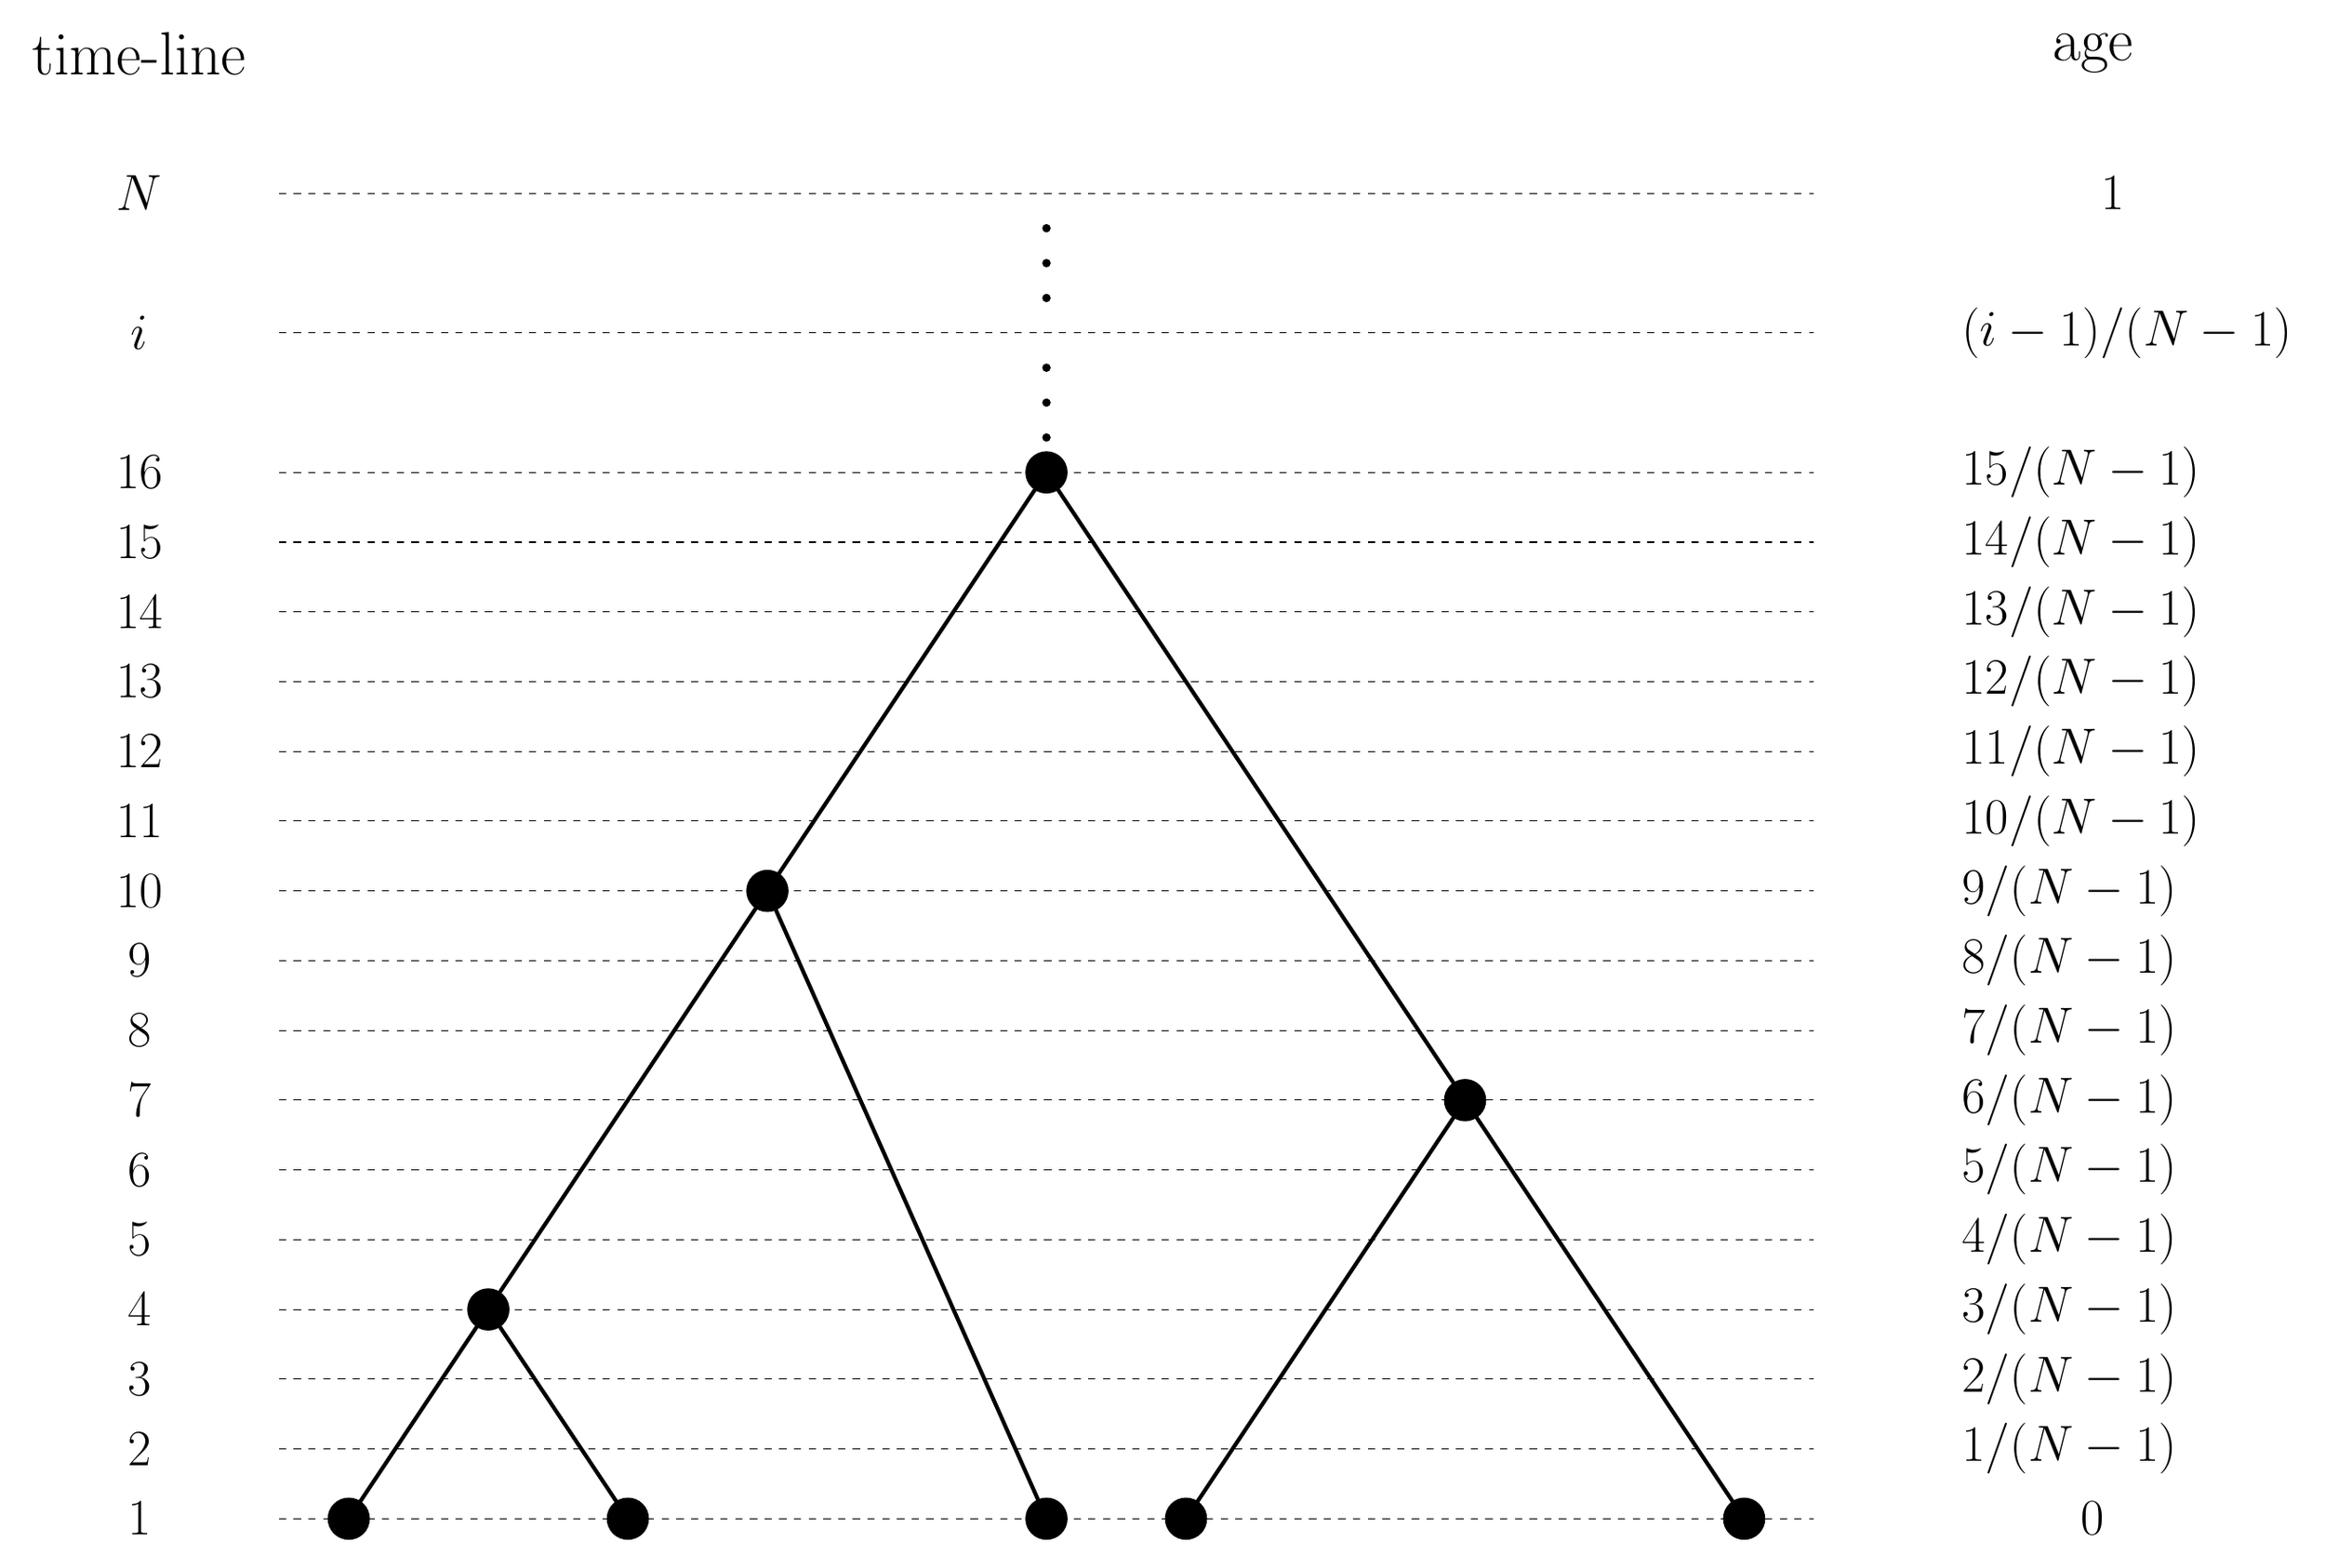
\begin{tikzpicture}[font=\Huge]
%\draw[step=1,gray,very thin] (0,0) grid (22,18);

\coordinate (a) at (11,16);

\coordinate (a1) at (11,1);
\coordinate (a2) at (1,1);

\coordinate (t1) at (3,4);
\fill (t1) circle (2ex);
\coordinate (t2) at (5,1);
\fill (t2) circle (2ex);
\draw[ultra thick] [-] (t1) -- (t2);

\fill (a) circle (2ex);
\fill (a1) circle (2ex);
\fill (a2) circle (2ex);

\draw[ultra thick] [-] (a) -- (a2);

\coordinate (b) at (7,10);
\fill (b) circle (2ex);
\draw[ultra thick] [-] (b) -- (a1);


\coordinate (a4) at (17,7);
\fill (a4) circle (2ex);

\coordinate (a5) at (13,1);
\fill (a5) circle (2ex);
\draw[ultra thick] [-] (a4) -- (a5);

\coordinate (a3) at (21,1);
\fill (a3) circle (2ex);
\draw[ultra thick] [-] (a) -- (a3);

% time-lines

\foreach \i in {1,...,16}
{
  \draw[dashed] [-] (0,\i) -- (22,\i);
}
  \draw[dashed] [-] (0,18) -- (22,18);
  \draw[dashed] [-] (0,20) -- (22,20);

% fill the ellipsis between time-line i

\fill (11,16.5) circle (0.4ex);
\fill (11,17) circle (0.4ex);
\fill (11,17.5) circle (0.4ex);


\fill (11,18.5) circle (0.4ex);
\fill (11,19) circle (0.4ex);
\fill (11,19.5) circle (0.4ex);

% time-line labels

\node at (-2,22) {time-line};
\foreach \i in {1,...,16}
{
  \node[font=\huge] at (-2,\i) {\i};
}

\node[font=\huge] at (-2,18) {$i$};

\node[font=\huge] at (-2,20) {$N$};

% ages

\node at (26,22) {age};

\node[font=\huge] at (26,1) {$0$};
\foreach \i in {1,...,15}
{
  \node[font=\huge,anchor=west] at (24,\i + 1) {$\i/(N-1)$};
}
\node[font=\huge,anchor=west] at (24,18) {$(i-1)/(N-1)$};
\node[font=\huge,anchor=west] at (26,20) {$1$};

\end{tikzpicture}
}
\caption{Tree $T$ mapped to $N$ discretized time-lines. Column `age' indicates
the date of each time-line in relative time units.}
\label{fig:mapping}
\end{figure}
%
%%%\ejmcomment{Not true in case of tip dating, but still currently true. 
%%%Also - we have some inconsistency on whether they are mapped to line 0 or 1.
%%%In the code it is 1 currently.}
%%% TOMAS: For simplicity, I changed the section to describe relative dating only and then
%%% extend it in the next section with fossil information. Therefore, I left property 2 intact.

Before describing the algorithm, it is necessary to define the interval $d(u)$ {\bf why would we call an interval d()?} of
discretized time-lines a node can be placed on, such that Property 1 holds {\bf not clear what property one refers to! is this from (i) or (ii) above?}. The
interval $d(r)$ for root $r$ is defined as 
$$d(r) = \{ i\ |\ h(r) \leq i <N\}$$ and for an arbitrary node $u$ as $$d(u) = \{ i\ |\ h(u) \leq i < \max
d(p); (p,u) \in E\}.$$ 
{\bf TODO Maybe describe all this in times like earliest = N with latest = 1 time line, I think this owuld be more intuitive to understand}
This is justified by the fact that the longest {\em path} from node $u$ leading to a leaf is of size $h(u)$ and contains exactly
$h(u)$ nodes (including $u$).  Therefore, we need to use at least $h(u)$ time-lines
for placing each node of this longest path onto a distinct, discrete time-line $i$.  
Hence, the first (most recent) time-line $u$ can be placed on, is $h(u)$. 
The same holds for the path from
$u$ to the root node $r$.  Each node on the path must be placed onto a distinct
time-line, and as such, the last (furthest back in time) time-line $u$ can be placed on, is the
one before {\bf TODO I'd rather write after here} the latest time-line its parent node $p$ can be placed on. The intervals for each
node can be computed by a preorder traversal of the tree.
Once this is done, one can maximize the score of equation (\ref{eq:score}) by splitting $f(T\ |\ n, \phi)$ into two terms
$f_1(T\ |\ n,\phi(r))$ and $f_2(T\ |\ \phi)$
%
%
\begin{equation}\label{eq:part1} 
f_1(T\ |\ n,\phi(r)) = n (\lambda-\mu)
                       \frac{(\lambda\rho)^{n-1}% 
                             (\lambda-\mu)^{2n-2}% 
                             e^{-(\lambda-\mu)\tau_{\phi(r)}}}%
                            {\rho\lambda +%
                             (\lambda(1 -\rho)-\mu)%
                             e^{-(\lambda-\mu)\tau_{\phi(r)}}}
\end{equation}
%
%
\begin{equation}\label{eq:part2}
f_2(T\ |\ \phi) = \prod_{u\notin L(T)}
                  \underbrace{
                    \frac{e^{-(\lambda-\mu)\tau_{\phi(u)}}}
                         {(\rho\lambda + 
                          (\lambda(1-\rho)-\mu)
                          e^{-(\lambda-\mu)\tau_{\phi(u)}})^2}
                  }_{\textrm{birth-death process term } b(\phi(u))}
                  \underbrace{
                    \gamma(\frac{\ell_{u,v}}{\tau_{\phi(u)}-\tau_{\phi(v)}})
                    \gamma(\frac{\ell_{u,w}}{\tau_{\phi(u)}-\tau_{\phi(w)}})
                  }_{\textrm{edge priors}}
\end{equation}
%
%
and computing all $|d(r)|$ maximum scores of 
$f_2(T\ |\ \phi_i), h(r) \leq i \leq N$, that is, for each time-line the root can be placed on. 
Because $f_1(T\ |\ n,\phi)$ depends only on the root time-line, the optimal mapping $\phi_i$ that
maximizes \ref{eq:score} (denoted by $\hat\phi$) is the one that leads to the
highest value of the product $f_1(T\ |\ n,\phi_i)\times f_2(T\ |\ \phi_i)$.%
Our approach is to maximize the term \ref{eq:part2} using a dynamic programming
algorithm. For that, we transform formula \ref{eq:part2} into
the following equivalent form, 
%
%
\begin{equation}\label{eq:DP}
\begin{split}
s(u\notin L(T),i) = %& \overbrace{\frac{e^{-(\lambda-\mu)\tau_i}}
                    %                  {(\rho\lambda + 
                    %                   (\lambda(1-\rho)-\mu)
                    %                   e^{-(\lambda-\mu)\tau_i})^2}
                    %  }^{\textrm{birth-death term } b(i)}\times\\
                    b(i)
                    %& 
                    \underbrace{
                        \max\{ s(v,j)\gamma(\frac{\ell_{u,v}}{\tau_i - \tau_j})\ |\ 
                          h(v) \leq j < i\}
                      }_{\textrm{max score of left child}}
                    %&
                    \underbrace{
                        \max\{ s(w,k)\gamma(\frac{\ell_{u,w}}{\tau_i - \tau_k\vphantom{\tau_j}})\ |\ 
                          h(w) \leq k < i\}
                      }_{\textrm{max score of right child}}\\
\end{split}
\end{equation}
%
%
where $s(u\in L(T),1) := 1$ for tip nodes.
{\bf TODO still not clear if this is DP or DP-like!}
The DP traverses the target tree in postorder and for each inner node $u$, it
computes a total of $|d(u)|$ maximized values $s(u,i), h(u) \leq i < h(u) + |d(u)|$, one
for each time-line on which node $u$ can be placed.  The score $s(u,i)$ of a
particular time-line $i$ of node $u$ is computed by finding the respective 
optimal time-lines $j$ and $k$ of its two children $v$ and $w$, which maximize the products of
$s(u,j)$ and $s(w,k)$ with the probability densities of the respective factorized edge
priors  $\gamma(\frac{\ell_{u,v}}{\tau_{i}-\tau_{j}})$ and
$\gamma(\frac{\ell_{u,w}}{\tau_{i}-\tau_{k}})$.
                    Note that, for a pair of time-lines $i$
and $j$ (resp.~$k$), we can factorize the branch length of edge $(u,v)$ 
(resp.~$(u,w)$) into a product of time (age) and rate.

This requires ${\cal O}((|d(v)|+|d(w)|)\times|d(u)|)$ computations for
determining the $|d(u)|$ optimal scores (and mappings) for $T_u$. These optimal
values for each time-line {\bf time line of u?} {\bf not entirely clear how time lines are linked to nodes here} 
are then stored in a table together with the positions (time-lines) of the two direct descendants (children).
This procedure is recursively applied to each tree node via a postorder tarversal 
(starting from the leaves and moving towards the root). Finally, once we have computed the terms
$s(r,i)$ {\bf say once more what they mean} for each possible time-line of the root node, we 
multiply them with the corresponding term $f_1(T\ |\ n, \phi(r))$, and select the root 
time-line that yields the optimal score.

{\bf TODO General: we should use optimal instead of maximal, consistently for clarity}

Thereafter, we initiate a backtracking process to calculate the optimal mapping $\hat\phi$. 
By selecting the optimal score (and hence the time-line of the root) we automatically obtain the time-lines of its two children, and,
at each of the two children, the time-lines of their respective children. Via recursion 
we thus obtain the time-lines of all nodes that maximize term \ref{eq:score}.

Fig.~\ref{fig:dp} depicts the bottom-up phase of the algorithm. 
The input is: the tree $T$ and the number of grid time-lines $N$.
{\bf what about the model parameters, state where you will discuss the choice and impact of parameter N}
In the first invocation $u$ is the root $r$ of the tree.  
The function returns three two-dimensional tables $M, M^r$, and
$M^l$, where entry $M(u,i), \min d(u) \leq i \leq \max d(u)$ contains the
optimal score for placing node $u$ onto time-line $i$.
The tables $M^r(u,i)$ and $M^l(u,i)$ copntain the optimal time-lines for 
the two children $v$ and $w$ with respect to the optimal score in $M(u,i)$. 
The algorithm is executed for each node via a post-order {\bf inconsistent writing, previsouly you always wrote postorder and preorder etc.} 
traversal in lines 7 and 11. 
%AS: this is trivial we can omit it. where in the case
%of an inner node, the function recursively calls itself with the node's left
%resp. right child as parameter. 
When the recursion reaches a tip node $v$
(resp. $w$), we set the table entries $M(v,1)$ and $M(w,1)$ to the
constant value $1$. The process then continues in a
bottom-up direction. 
{\bf TODO the following paragraph needs to be entirely re-written ins simpler language, shorter sentences, fewer grammatical errors and less passive forms!}
 As soon as the entries of table $M$ have been computed for the
two children of an inner node $u$, the algorithm computes all entries
(time-lines) $M(u,i), \min d(u) \leq i \leq \max d(u)$ for node $u$ (lines
12-25) by finding the maximal product among all scores $M(v,j), \min d(v) \leq j
< i$ resp. $M(w,k), \min d(w) \leq k < i$ of time-lines each child $v$ (lines
14-17) resp. $w$ (lines 18-21) could have been placed on given by the current
time-line $i$ of $u$, multiplied by the prior of factorized edge rates
$\ell_{u,v}/(\tau_i - \tau_j)$ resp. $\ell_{u,w}/(\tau_i - \tau_k)$. Once the
maximal products for $v$ and $w$ are found (denoted as $\hat f_v$ resp. $\hat
f_w$), the score of time-line $i$ for node $u$ is computed as their product
multiplied by the birth-death term $b(i)$ and stored in $M(u,i)$ (line 22).
The time-lines of $v$ resp. $w$ which yielded $\hat f_{v}$ resp. $\hat f_{w}$
are stored in $M^l(u,i)$ resp. $M^r(u,i)$ (line 23). In addition, if node $u$
is the root, it is multiplied by the term $f_1(T\ |\ n,i)$ (line 25).

\setcounter{instr}{0}
\begin{figure}[t]
\begin{center}
\renewcommand*\arraystretch{.5}
\begin{tabular}{|rl|}
\hline
\multicolumn{2}{|l|}{\textsc{DP}$(T, N, u)$}\\
\ninstr & $v \leftarrow$ left child of $u$\\
\ninstr & $w \leftarrow$ right child of $u$\\
\ninstr & $r \leftarrow$ the root of $T$\\
\ninstr & \textbf{if} $v \in L(T)$ \textbf{then}\\
\ninstr & \qquad $M(v,1) \leftarrow 1$\\
\ninstr & \qquad \textbf{return}\\
\ninstr & \textsc{DP}(T,N,v)\\        
\ninstr & \textbf{if} $w \in L(T)$ \textbf{then}\\
\ninstr & \qquad $M(w,1) \leftarrow 1$\\
\ninstr & \qquad \textbf{return}\\
\ninstr & \textsc{DP}(T,N,w)\\        
\ninstr & \textbf{for} $i \leftarrow \min d(u)$ \textbf{to} $\max d(u)$ \\
\ninstr & \qquad $\hat{f}_v \leftarrow 0, \hat{f}_w \leftarrow 0$ \\
\ninstr & \qquad \textbf{for} $j \leftarrow \min d(v)$ \textbf{to} $i-1$ \\
\ninstr & \qquad \qquad  \textbf{if} $\gamma(\ell_{u,v}/(\tau_i - \tau_j))  s(v,j) > \hat{f}_v$ \textbf{then} \\
\ninstr & \qquad \qquad \qquad $\hat{f}_v \leftarrow \gamma(\ell_{u,v}/(\tau_i - \tau_j))  s(v,j)$\\
\ninstr & \qquad \qquad \qquad $\hat j \leftarrow j$\\
\ninstr & \qquad \textbf{for} $k \leftarrow \min d(w)$ \textbf{to} $i-1$ \\
\ninstr & \qquad \qquad  \textbf{if} $\gamma(\ell_{u,w}/(\tau_i-\tau_k))  s(v,k) > \hat{f}_w$ \textbf{then} \\
\ninstr & \qquad \qquad \qquad $\hat{f}_w \leftarrow \gamma(\ell_{u,w}/(\tau_i-\tau_k))  s(w,k)$\\
\ninstr & \qquad \qquad \qquad $\hat k \leftarrow k$\\
\ninstr & \qquad $M(u,i) \leftarrow b(i) \times \hat f_{v} \times \hat f_{w}$\\
\ninstr & \qquad $M^l(u,i) \leftarrow \hat j, M^r(u,i) \leftarrow \hat k$\\
\ninstr & \qquad \textbf{if} $u = r$  \textbf{then}\\
\ninstr & \qquad \qquad $M(u,i) \leftarrow M(u,i) \times f_1(T\ |\ n,i)$ \\

\hline  
\end{tabular}
\end{center}
\caption{The bottom-up phase of the DP algorithm for computing relative
divergence times. The algorithm accepts three parameters; tree ($T$), number of
discretization lines ($N$) and the root $u$ of subtree  $T_u$. In it's first
call, the root $r$ of $T$ is passed as $u$.  It recursively traverses the tree
in postorder and constructs a table $M$ of the optimal scores for each node $u$
and time-line $i$, where $\min d(u) \leq i \leq \max d(u)$, along with
information on how to retrieve the optimal mapping $V$ in the later,
backtracking phase (not in Figure).}
\label{fig:dp}
\end{figure}

W.l.o.g we now prove that the DP algorithm computes the optimal score of
\ref{eq:part2} given the grid size $N$ and the values of $\lambda,\mu,\rho$.

\begin{theorem}[Optimality of DP]
Given the number of discretization intervals, the values of $\lambda,\mu,\rho$,
Algorithm DP computes the optimal score of (\ref{eq:score}).
\end{theorem}
\begin{proof}
We show that the score terms $s(r,i), h(r) \leq i \leq N$ the DP computes are
in fact equal to $f_2(T,\hat\phi_i)$ and hence, finding the product
$f_2(T,\phi_i)\times f_1(T,\phi_i)$ that yields the highest value represents the
optimal solution. We prove this by strong induction on the height of the
root node.
\paragraph{Base case.} Let $u$ be the parent of $v$ and $w$, such that $h(u) =

1$. {\bf how can h of a non-tip node u be 1?} 
Nodes $v$ and $w$ 
are therefore leaves, such that we have to compute

$|d(u)|=N-1$ values, of the form
%
%
$$
s(u,i) = b(i)
         \gamma(\frac{\ell_{u,v}}{\tau_i})
         \gamma(\frac{\ell_{u,w}}{\tau_i})
$$
%
%
for each $i \in d(u)$. Since DP selects the score that maximizes the product
when multiplied with $f_1(T,\phi)$, we obtain the optimal score.
\paragraph{Inductive step.} Assume the claim holds for each node $u$ of height
$1 \leq h(u) \leq m$. Our task is to prove that the claim holds for $h(u) =
m+1$.  According to the definition of $h()$, a node $u$ of height $h(u)=m+1$
has a child $v$ of height $h(v)=m$ and a child $w$ of height $0 \leq h(w) \leq
m$.  Since the values $s(v,j), h(v) \leq j \leq \max d(v)$ and $s(w,k), 1 \leq
k \leq \max d(w)$ are maximized (assumption), we compute $|d(u)|$ values
%
%
\begin{equation*}
\begin{split}
s(u,i) =  b(i)\times 
          \max\{ s(v,j)\gamma(\frac{\ell_{u,v}}{\tau_i-\tau_j})\ |\
              h(v) \leq j < i\} \times 
          \max\{ s(w,k)\gamma(\frac{\ell_{u,w}}{\tau_i-\tau_k})\ |\ 
               h(w) \leq k < i\}
\end{split}
\end{equation*}
%
%
and select the optimal.
\qed\end{proof}

\section{Extending the DP algorithm with node prior information}
\textbf{Not finished yet.} Node priors are either log-normal or exponential
distributions together with an {\em offset} $\varphi$ (minimum age).  The
algorithm is the same as in ``relative dating'' except that it is also given a
theoretical maximum age $\zeta$ for line $N$ of the grid.  When running the DP
algorithm for the time-line $i$ of an inner node $u$ that is calibrated with a
distribution, then Equation (\ref{eq:score}) is multiplied by the probability
density function of its distribution for value $\tau_i \times \zeta - \varphi$,
and with $1$ otherwise.

\section{Extending the DP algorithm with tip date information}
To come

\section{Description of software}
Maybe in supplement? 
{\bf TODO, need to see, if it is just a straight-forward implementation of the recursion and equations and can go into the supplement}
%FastDate requires as input a fully bifurcating rooted phylogeny with branch lengths,
%and user defined estimates of birth rate ($\lambda$), death rate ($\mu$), 
%and proportion of descendants of the most recent common ancestor of the taxa found in the tree
%which were sampled in the tree ($\rho$).
%In addition a rate mean ($\bar{r}$) and a rate variance ($\sigma$) must be provided by the user
%to parameterize the gamma prior on branch rates.

\section {Auto-correlated rates}


\subsection{Relative dating}
For relative dating estimates (generating an ultrametric tree), a number or
intervals ($N$) my be provided to control the granularity of the relative age
estimates.


\subsection{Node prior}
The user can input prior information on node dates in the form of an exponential
or log normal distribution, and a minimum age offset.



\subsection{Tip dating}
\ejmcomment{not yet fully implemented}
Optional parameters include $\psi$ the rate of recovery of fossils per lineage, 
if extinct tips have been sampled. {\bf this is the first time you actually define $\psi$}



\section{Examples}
\subsection{Node dating example from 1 KITE}

\subsection{Other tip dating test data from LSD?}

\subsection{dating of that science paper}

\section{Discussion}

TODO Compare to Gascuel `LSD' and other rapid approaches.

{\bf TODO: discuss input parameter optimization, discuss choice of N, describe strtegy to automatically determine N, e.g., keep multiplying N by 2 until 
estimated parameters do not change significantly any more, sho some experiments of impact of N or propose default value}


\bibliographystyle{sysbio}
\bibliography{dating}
\end{document}
